\chapter{\label{Intro}Introduction}

The rendering problem of calculating radiance  (brightness) of surfaces in a 3 dimensional (3D) scene, to synthesize images of the scene, is very important in 3D computer graphics. Given the geometric and optical properties (BRDF, light source) of all surfaces in 3D scene, our concern is to calculate radiance function defined over all the surfaces and generate realistic looking image of the scene, from particular viewpoint, illuminated with light source in the scene.

\section{Direct and Indirect Illumination renderer}
A renderer, in computer graphics, is algorithm which synthesize images of a scene. There are two types of renderer, direct illumination renderer and indirect illumination renderer. 
\begin{figure}[tbh]
\centering{}
\captionsetup{justification=centering}
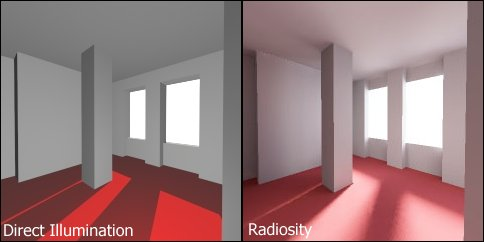
\includegraphics[width=5in]{DirectIndirect.jpg}
\caption{\label{fig:directindirect}Difference between images generated using direct illumination and indirect illumination renderer (radiosity)\\ \cite{wikiradiosity}}
\end{figure}
Figure \ref{fig:directindirect} shows differences between image synthesized by direct and indirect illumination . The image on the left is rendered with direct illumination renderer. All the surfaces are illuminated by light received directly from light source and ambient light without which surfaces which are not directly illuminated will be completely dark. Image on the right of Figure \ref{fig:directindirect} is rendered by indirect illumination renderer. We can see that the illumination of a surface is result of inter-reflection of light between surfaces. As a result we can see that the pink color of floor is blended with the white color of wall. This effect is called color blending, which is one of the feature of a realistic looking images.  We can see that image synthesized using indirect illumination renderer are more realistic than direct illumination renderer.

\section{Radiosity and Indirect Illumination renderer }

Global illumination or indirect illumination is a name for a class of algorithms  (renderer) used in 3D computer graphics that are meant to add more realistic lighting to 3D scenes as compared to direct illumination renderer. Such algorithms take into account not only the light which comes directly from a light source, but also light from the same source which is being reflected by other surfaces in the scene. As a result, global illumination adds realistic features like light bouncing  (multiple inter-reflection between two surfaces) and color bleeding between pair of surfaces. A well known global illumination algorithm is ray-tracing \cite{Whitted}, which computes  radiance of a area of a surface of a scene visible  from given viewpoint. In other words, it only calculates radiance of points which are visible in final image. Thus for changing the viewpoint of image of the scene, we need to run algorithm again, making the algorithm viewpoint dependent. Other set of global illumination algorithms is radiosity, which are viewpoint independent used for scene with diffused surfaces.


Radiosity algorithms are set of global illumination algorithms which are used for scenes with surfaces reflecting light diffusely (emitting equal brightness in all the directions above the surface apparently). In other words, radiosity takes 3D scenes with Lambertian surfaces as input. Lambertian reflectance is property of an ideal "matte" or diffusely reflecting surface. Opposite to ray-tracing, radiosity calculates radiance of all points in the scene. This allows the computation to be viewpoint independent i.e. solution for given scene can be used to synthesize images of scene from any arbitrary viewpoint. This is advantage as well as drawback as we need to do extra work to find radiance of all the points. \\

Radiosity also refers to measure of power per unit area at a point. Thus solution of the this problem is radiosity function over the domain of surfaces in the scene. our goal is to use projection methods used for solving radiosity integral equation. Reduce complexity and increase accuracy of numerically calculated solution of radiosity problem. Wavelets gives promising results with its property of vanishing 
moments. Thus use of projection methods with wavelets is termed as {\em wavelet radiosity} \cite{gortler}.


\section{Organization of the Report}
We first discuss literature survey and approaches taken to solve the problem of radiosity in Chapter \ref{ch:literature}. Then we formally define radiosity problem and associated radiosity integral equation, in Chapter \ref{ch:problemformulation}. Then projection methods, numerical methods, is discussed in Chapters \ref{ch:projection}, \ref{ch:wavelets} and \ref{ch:waveletprojection} with different basis and finite dimensional space discussed in Chapter \ref{ch:wavelets}. Finally we discuss results and comparison of wavelets in Chapter \ref{ch:experimentandresult}.